\begin{frame}\frametitle{$e\rightarrow\gamma$ Background. Source}

\end{frame}% end of \frametitle{Source}

\begin{frame}\frametitle{$e\rightarrow\gamma$ Background. Method Description}
{\footnotesize\bfseries{Method Description}}
\scriptsize
\begin{itemize}
  \item Get $N_{MC-Zpeak}^{e\rightarrow\gamma}$ (number of $e\rightarrow\gamma$ events under the Z-peak based on the MC prediction); done by counting
  \item Get $N_{data-Zpeak}^{e\rightarrow\gamma}$ (number of $e\rightarrow\gamma$ events under the Z-peak from data); done by fitting
  \item Get $N_{MC-nom}^{e\rightarrow\gamma}$ (number of $e\rightarrow\gamma$ events in the nominal range based on the MC prediction); done by counting
  \item Get $N_{data-nom}^{e\rightarrow\gamma}$ (number of $e\rightarrow\gamma$ events in the nominal range based on the MC predictionfrom data); done by scaling {\footnotesize\bfseries{$N_{data-nom}^{e\rightarrow\gamma} = N_{MC-nom}^{e\rightarrow\gamma} \cdot N_{data-Zpeak}^{e\rightarrow\gamma}/N_{MC-Zpeak}^{e\rightarrow\gamma}$}}
\end{itemize}
\end{frame}% end of \frametitle{Method Description}

\begin{frame}\frametitle{$M_{e,\gamma}$ Fit Model and Fit Plots. 15-20 GeV, barrel}
\scriptsize
$N_{sig} \cdot (RooNDKeysPdf~x~Gaussian) +  N_{bkg} \cdot (RooCMSShapePdf)$\\
\begin{figure}[htb]
  \begin{center}
   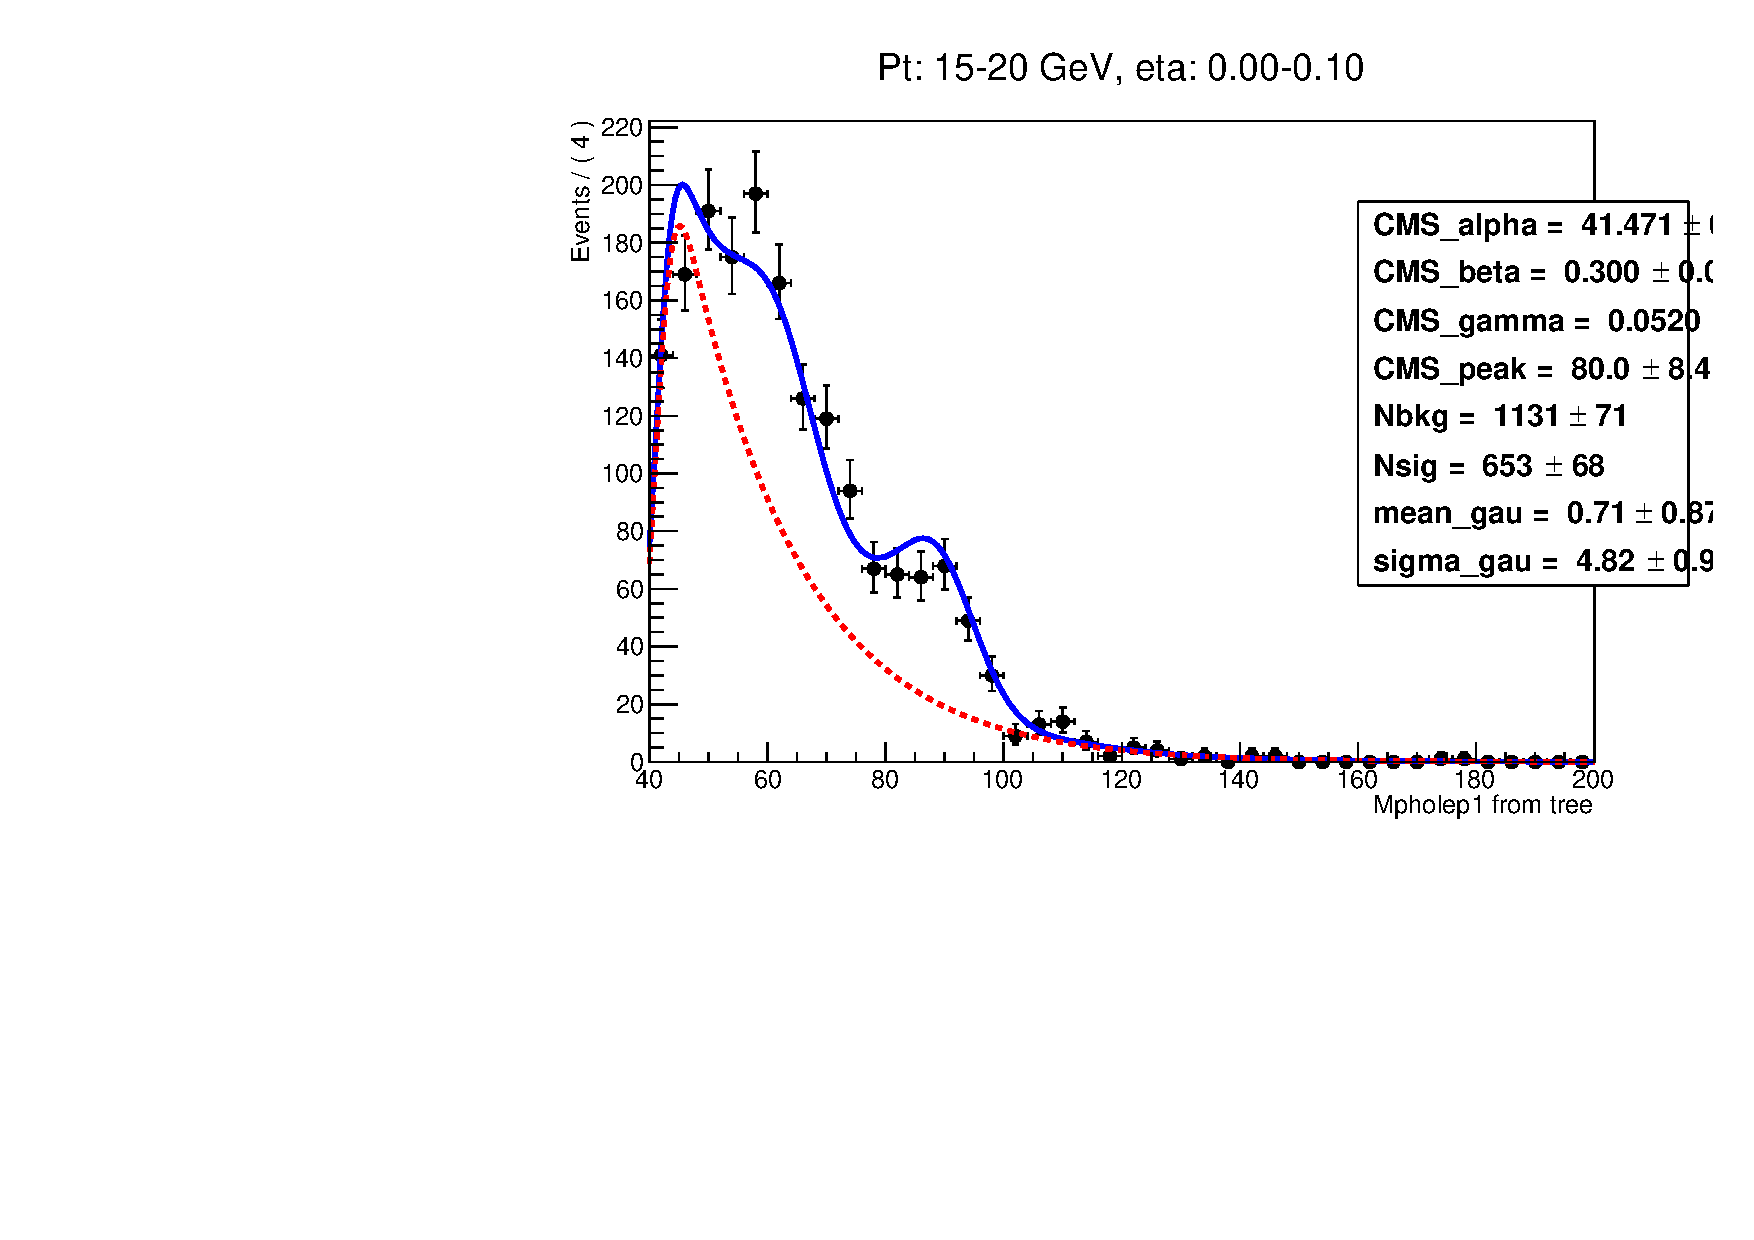
\includegraphics[width=0.25\textwidth]{../figs/figs_v11/ELECTRON_WGamma/EtoGammaFits/sa_hZmass_h_Data_EtoGamma_Enr_BARREL_pt15to20_ieta0.pdf}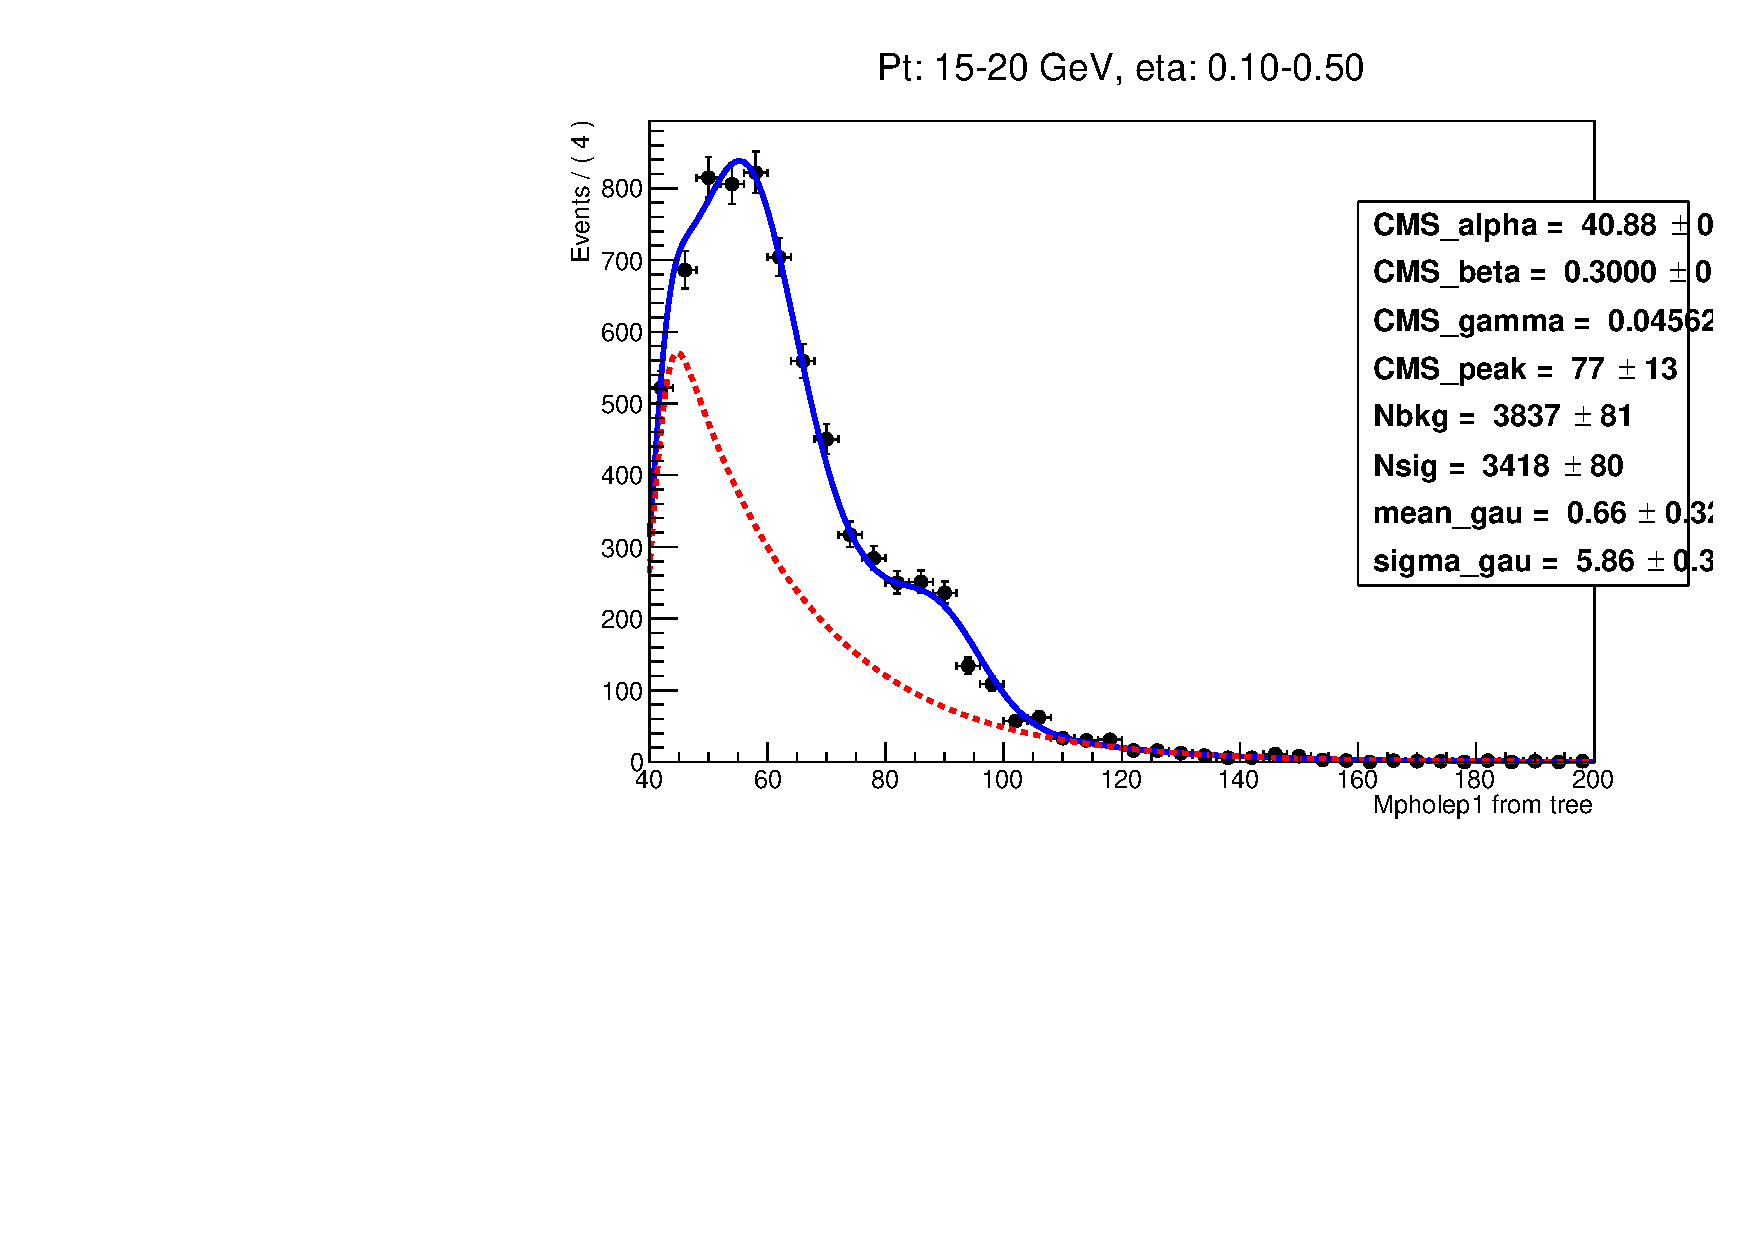
\includegraphics[width=0.25\textwidth]{../figs/figs_v11/ELECTRON_WGamma/EtoGammaFits/sa_hZmass_h_Data_EtoGamma_Enr_BARREL_pt15to20_ieta1.pdf}\\
   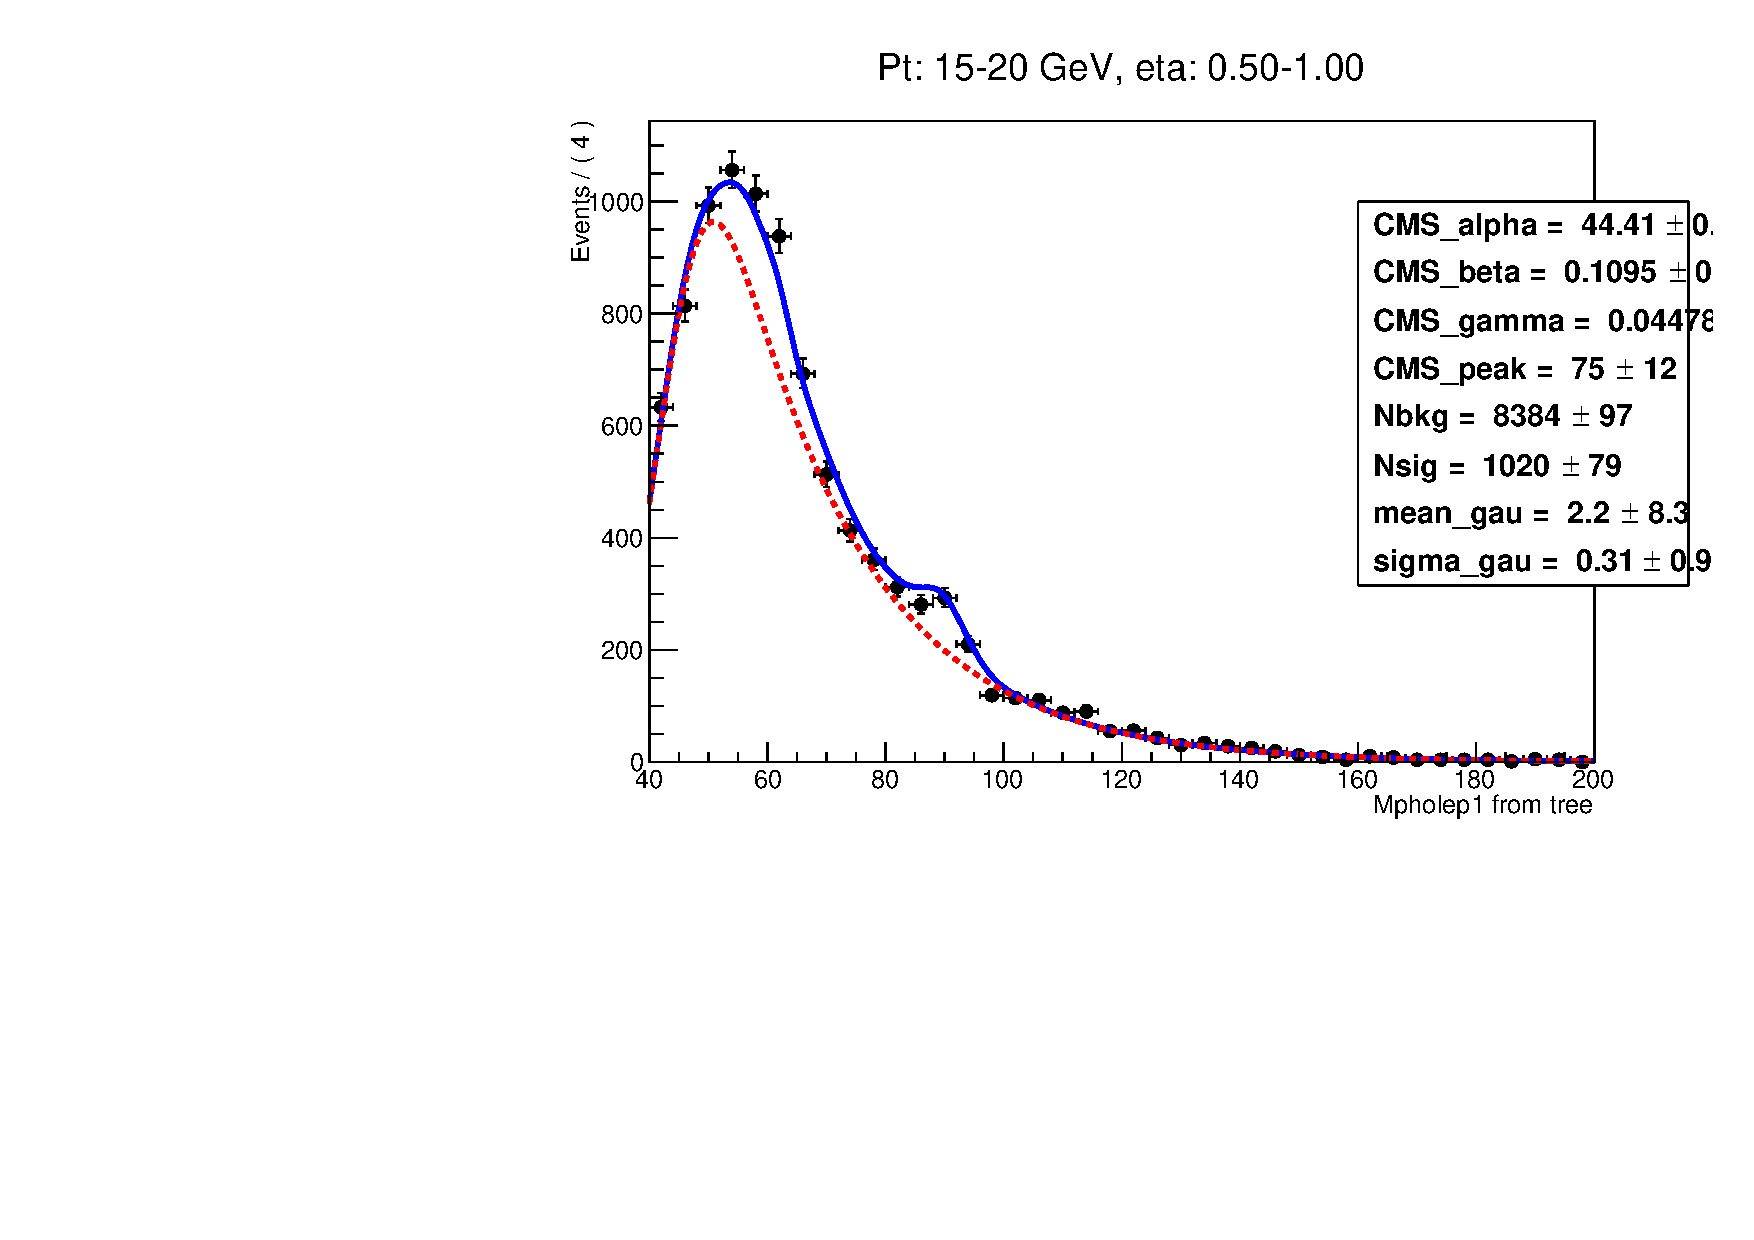
\includegraphics[width=0.25\textwidth]{../figs/figs_v11/ELECTRON_WGamma/EtoGammaFits/sa_hZmass_h_Data_EtoGamma_Enr_BARREL_pt15to20_ieta2.pdf}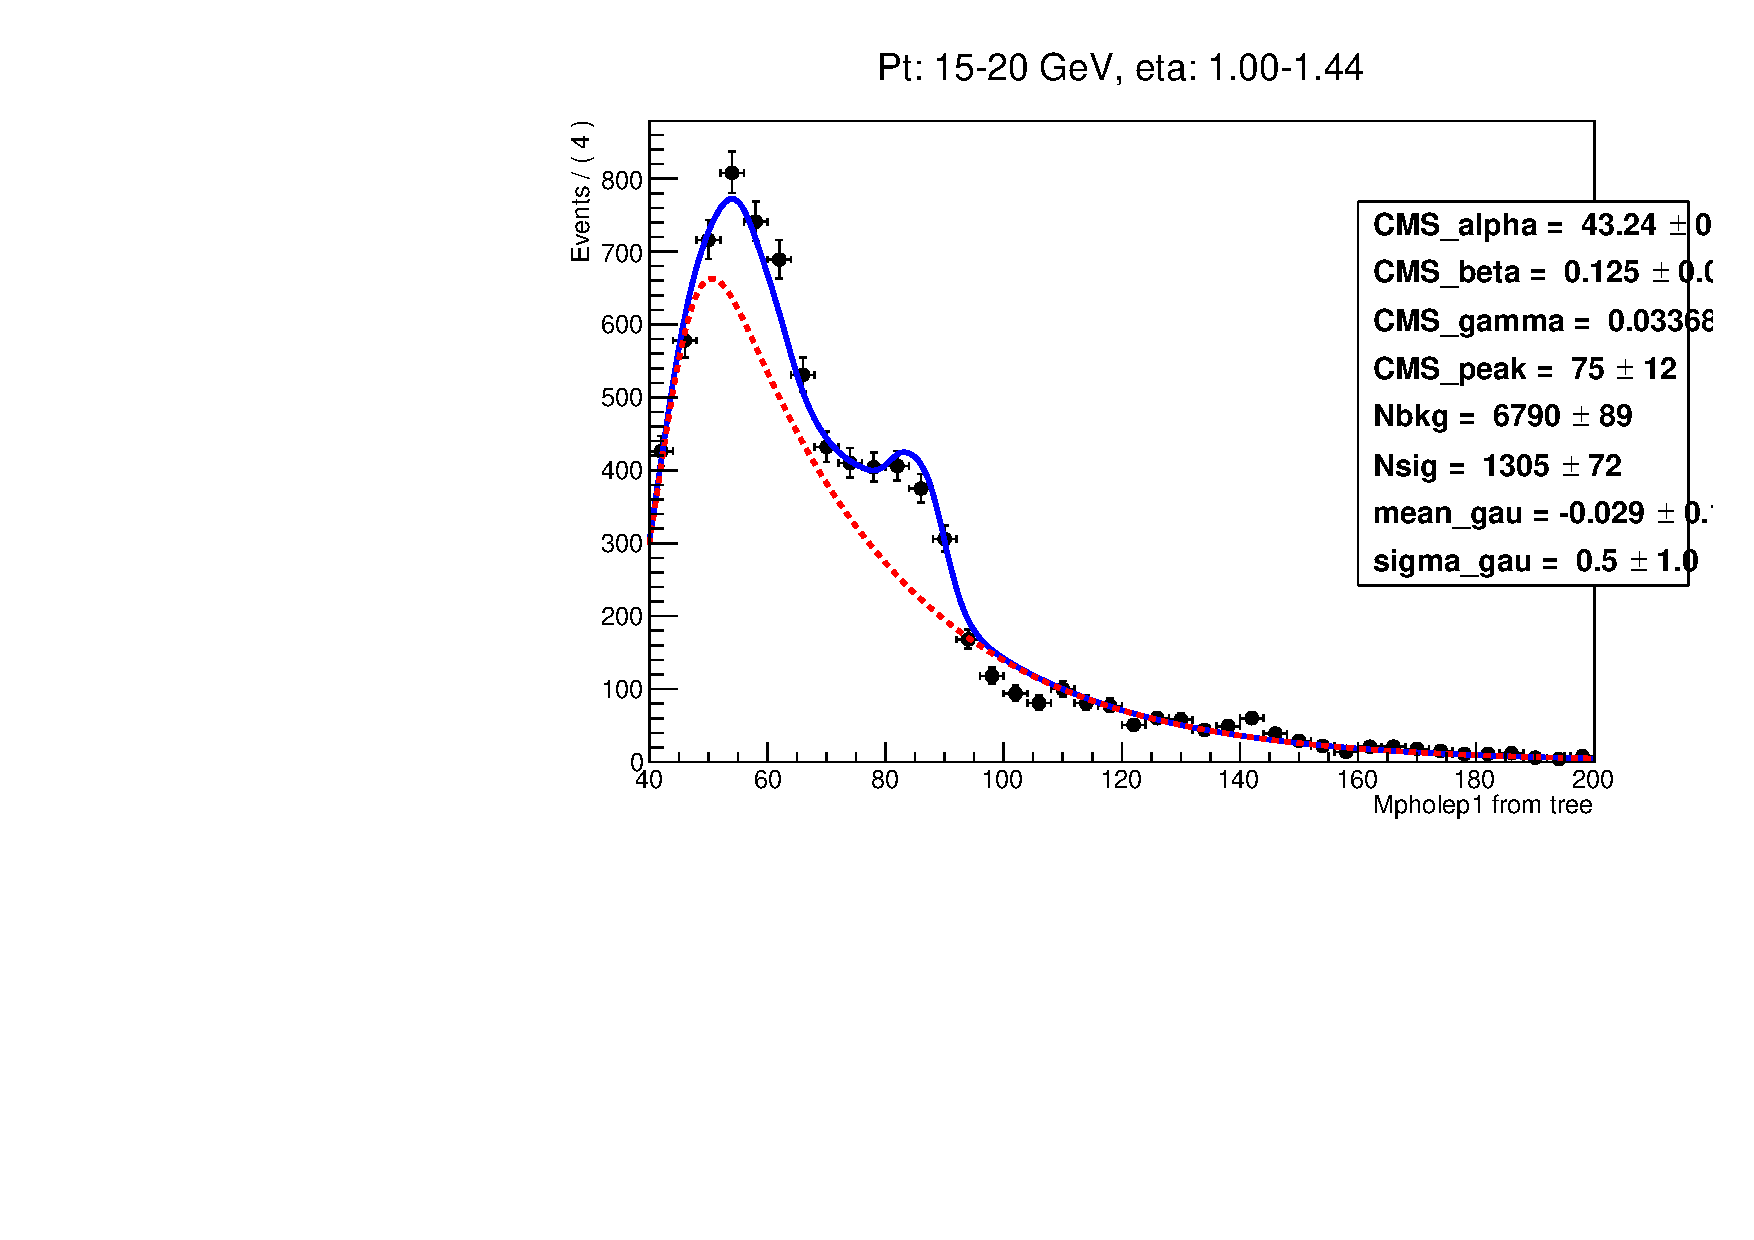
\includegraphics[width=0.25\textwidth]{../figs/figs_v11/ELECTRON_WGamma/EtoGammaFits/sa_hZmass_h_Data_EtoGamma_Enr_BARREL_pt15to20_ieta3.pdf}\\
  \caption{$M_{e,\gamma}$ fits, W$\gamma$, electron channel, 15-20 GeV, barrel, 4 eta bins}
  \end{center}
\end{figure}
\end{frame}%\frametitle{$M_{e,\gamma}$ Fit Plots. 15-20 GeV, barrel}
